\subsection{Prospects at Run-3}
\begin{frame}{Prospects at Run-3}

\begin{columns}
\column{0.6\textwidth}

\begin{itemize}
    \item Extrapolate to $\sim$ 300 fb$^{-1}$, $\sqrt{s}$ increase neglected
    \item Detector upgrades: \textbf{no impact on HH$\to b\bar{b}\gamma\gamma$}
\end{itemize}
\onslide<2->{
\begin{itemize}
    \item $\frac{\sigma_{HH}}{\sigma_{HH}^{SM}}$ limit: \textcolor{HHred}{\textbf{3.8}} (\textcolor{cadmiumorange}{\textbf{1.4 $\times$ imp.}} w.r.t 139 fb$^{-1}$)
\end{itemize}
\begin{table}
    \centering
    \begin{tabular}{lcc}
    \hline\hline
        Scenario & 1$\sigma$ CI & 2$\sigma$ CI  \\
        \hline
        Run-2 & [-1.3, 6.4] & [-2.9, 8] \\
        Run-3 & \textbf{[-0.7, 5.6]} & \textbf{[-1.9, 7]} \\
        \hline\hline
    \end{tabular}
\end{table}
}
\onslide<3->{

\underline{Potential improvements}:
\begin{itemize}
    \item \textbf{DNN categorization}: \textcolor{HHred}{\textbf{$\sim$10\%}}
    \item $m_{b \bar{b}}$ imp. with \textbf{kinematic fit}: \textcolor{HHred}{\textbf{2-5\%}}
    \item \textbf{photon identification}: \textcolor{HHred}{\textbf{7\%}}
\end{itemize}
}
\column{0.4\textwidth}

\visible<2-3>{
\begin{figure}
    \centering
    \fcolorbox{HHred}{HHwhite2}{
    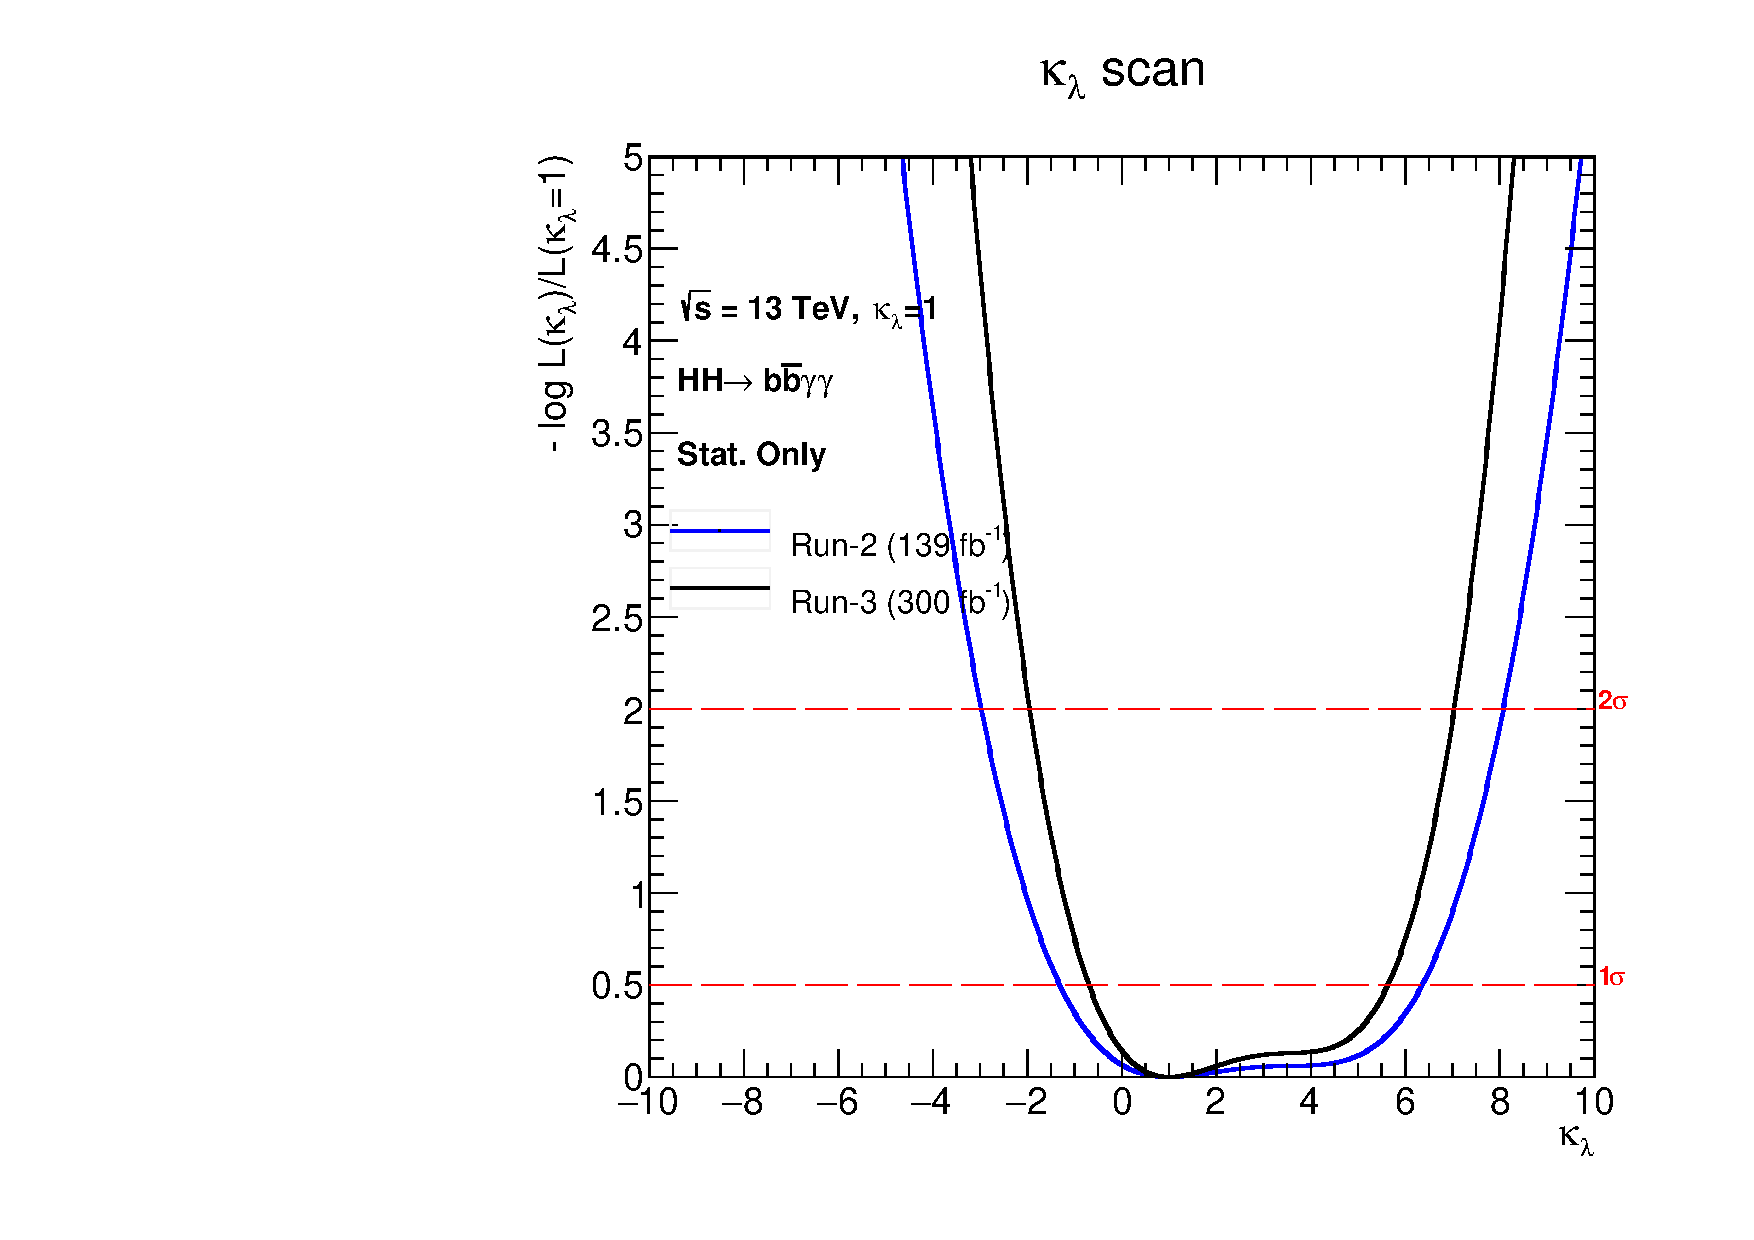
\includegraphics[width=1\textwidth]{Part4/Img/likelihood_subplot_Run3.pdf}
    }
\end{figure}
}
\end{columns}
\end{frame}

\subsection{Prospects at HL-LHC}
\begin{frame}{Prospects at HL-LHC}

\begin{columns}
\column{0.4\textwidth}

\begin{figure}
    \begin{overprint}
    \onslide<1>\centering\fcolorbox{HHturquoise_d}{HHwhite2}{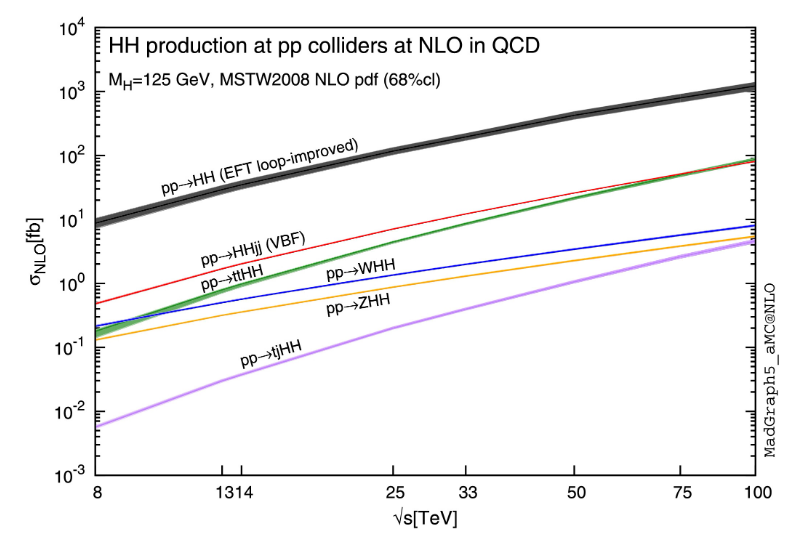
\includegraphics[width=1\textwidth]{Part1/Img/HH_XSec_as_S.png}}
    \onslide<2-3>\centering\fcolorbox{HHred}{HHwhite2}{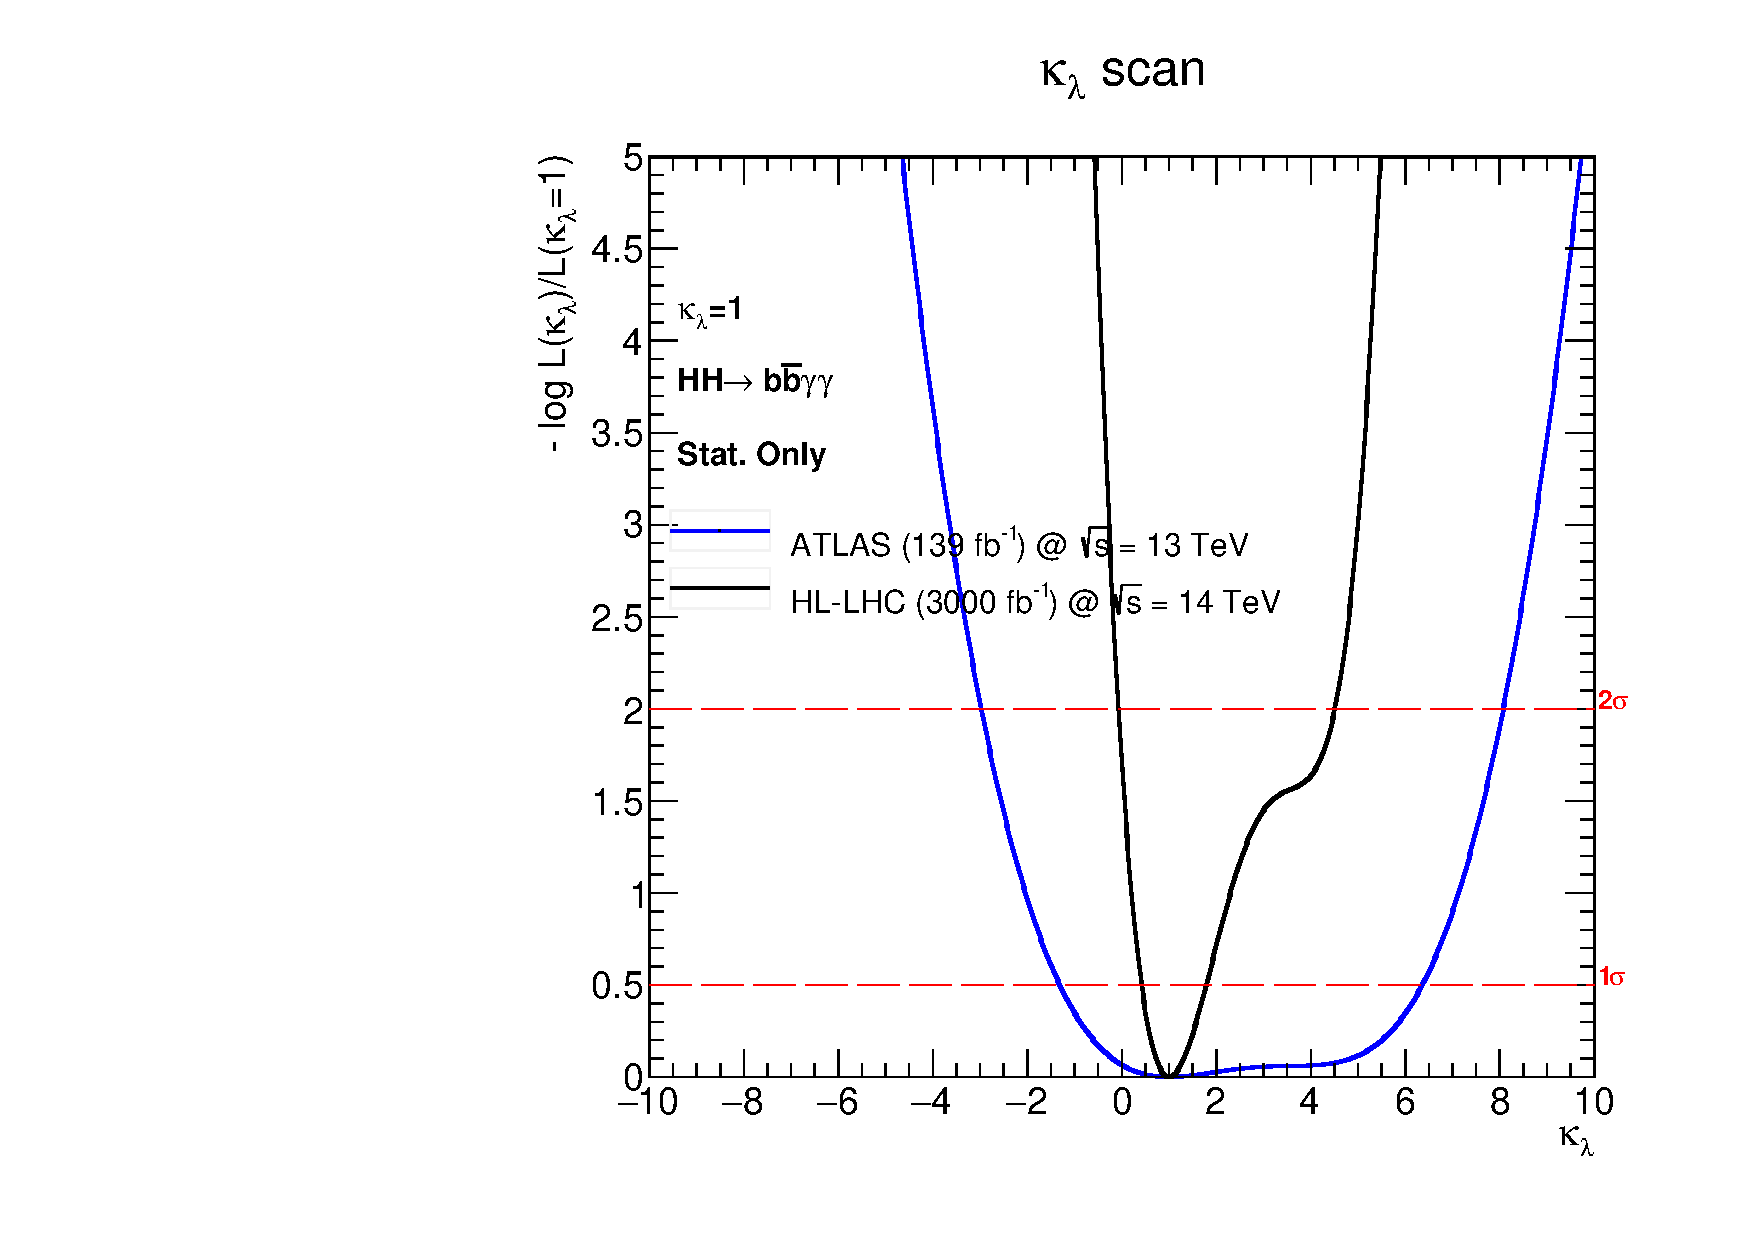
\includegraphics[width=1\textwidth]{Part4/Img/likelihood_subplot_14TeV.pdf}}
   \end{overprint}
\end{figure}


\column{0.6\textwidth}
\begin{itemize}
    \item \textbf{Extrapolate to \textcolor{HHturquoise_d}{$\sim$ 3000 fb$^{-1}$ at 14 TeV}}
    \item European strategy (from 36 fb$^{-1}$) expects: 
    \begin{center}
       \textit{ \textcolor{gray}{ATLAS+CMS}}
    \end{center}
    \begin{itemize}
        \item Significance of \textbf{\textcolor{HHred}{4$\sigma$}}
        \item \textbf{$\kappa_{\lambda} = 1 \pm 50\%$ at 68\% CL}
    \end{itemize}
    \onslide<2-3>{
    \item Detector upgrades: \textbf{mitigate higher pileup} 
    }
\end{itemize}
\onslide<2-3>{
\begin{table}[]
    \centering
    \begin{tabular}{lcc}
        \hline\hline
        Scenario & 1$\sigma$ CI & 2$\sigma$ CI  \\
        \hline
        Run-2 & [-1.3, 6.4] & [-2.9, 8] \\
        European Strat. & [-0.1, 2.4] & [-1.1, 8.1] \\
        HL-LHC & \textbf{[0.4, 1.8]} & \textbf{[-0.1, 4.4]} \\
        \hline\hline
    \end{tabular}
\end{table}
}
\onslide<3>{
\begin{center}
    \textbf{\textcolor{HHred}{Large gain at high $\kappa_{\lambda}$}}
\end{center}
}
\end{columns}    
\end{frame}

\begin{frame}{Prospects at HL-LHC}

\begin{columns}
\column{0.4\textwidth}

\begin{figure}
  \centering
  \fcolorbox{HHturquoise_d}{HHwhite2}{
   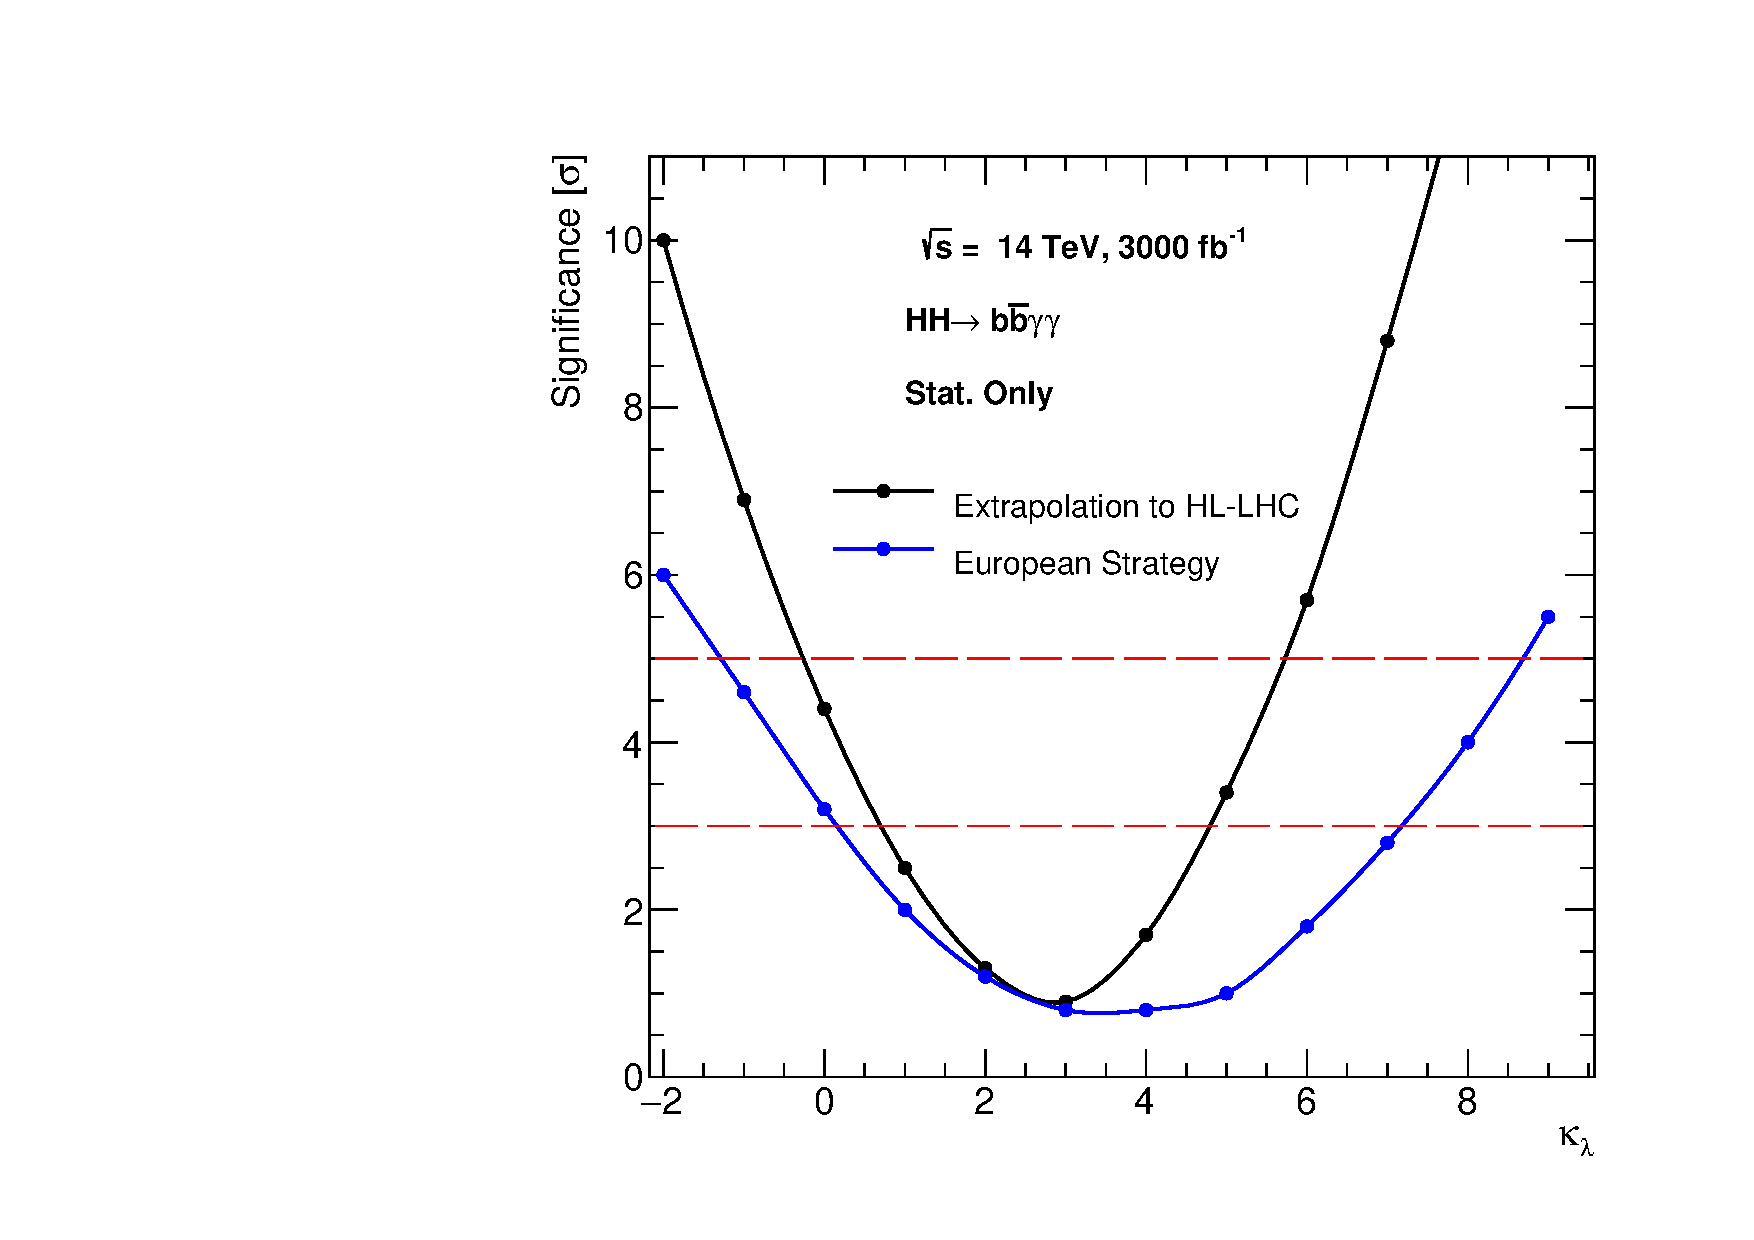
\includegraphics[width=1\textwidth]{Part4/Img/sig.pdf}
   }
\end{figure}


\column{0.6\textwidth}
\begin{itemize}
    \item Extrapolate to $\sim$ 3000 fb$^{-1}$ at 14 TeV
    \item European strategy (from 36 fb$^{-1}$) expects: 
    \begin{center}
       \textit{ \textcolor{gray}{ATLAS+CMS}}
    \end{center}
    \begin{itemize}
        \item Significance of \textbf{\textcolor{HHred}{4$\sigma$}}
        \item \textbf{$\kappa_{\lambda} = 1 \pm 50\%$ at 68\% CL}
    \end{itemize}
    \item Detector upgrades: \textbf{mitigate higher pileup effectss} 
\end{itemize}

\begin{table}[]
    \centering
    \begin{tabular}{lc}
        \hline\hline
        Scenario & Significance [$\sigma$]  \\
        \hline
        Run-2 & 0.48 \\
        European Strat. & 2.1 \\
        HL-LHC & \textcolor{HHturquoise_d}{\textbf{2.5}} \\
        \hline\hline
    \end{tabular}
\end{table}
\onslide<2>{
\begin{center}
    \textbf{\textcolor{HHturquoise_d}{Similar performance for SM} } \\
    \textbf{\textcolor{HHred}{Large gain at high $\kappa_{\lambda}$}}
\end{center}
}
\end{columns}  
\end{frame}